% ------------------------------------------------------------------------ %
% !TEX encoding = UTF-8 Unicode
% !TEX TS-program = pdflatex
% !TEX root = ../Tesi.tex
% !TEX spellcheck = it-IT
% ------------------------------------------------------------------------ %
%
% ------------------------------------------------------------------------ %
% 	NOME CAPITOLO
% ------------------------------------------------------------------------ %
%
\chapter{Prove Sperimentali}
%
\label{cap:provesperimentali}
%
% ------------------------------------------------------------------------ %
%
\section{Sezione}
La figura~\vref{fig:grafici} riporta alcuni grafici di esempio, creati con MatLab ed esportati in formato vettoriale (.eps), con griglia in ogni grafico, box esterno, e dimensione del font adeguata per la tesi stampata.
%
% SUB-FIGURE
% ------------------------------------------------------------------------ %
% grafici inventati
% ------------------------------------------------------------------------ %
%
\begin{figure}
%
\centering
%
\subfloat[][immagine1\label{fig:grafici-1}]
   {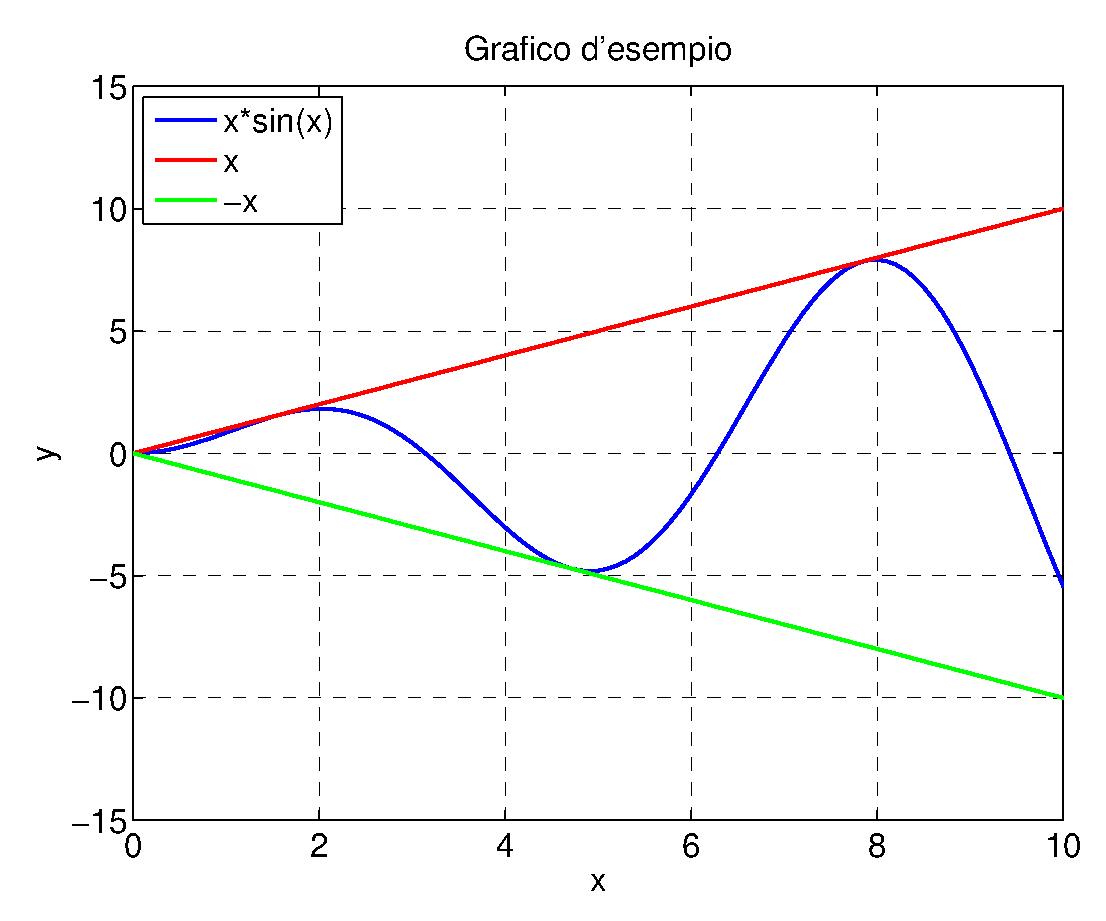
\includegraphics[width=.5\textwidth]{immagine1}}
%
\subfloat[][immagine2\label{fig:grafici-2}]
   {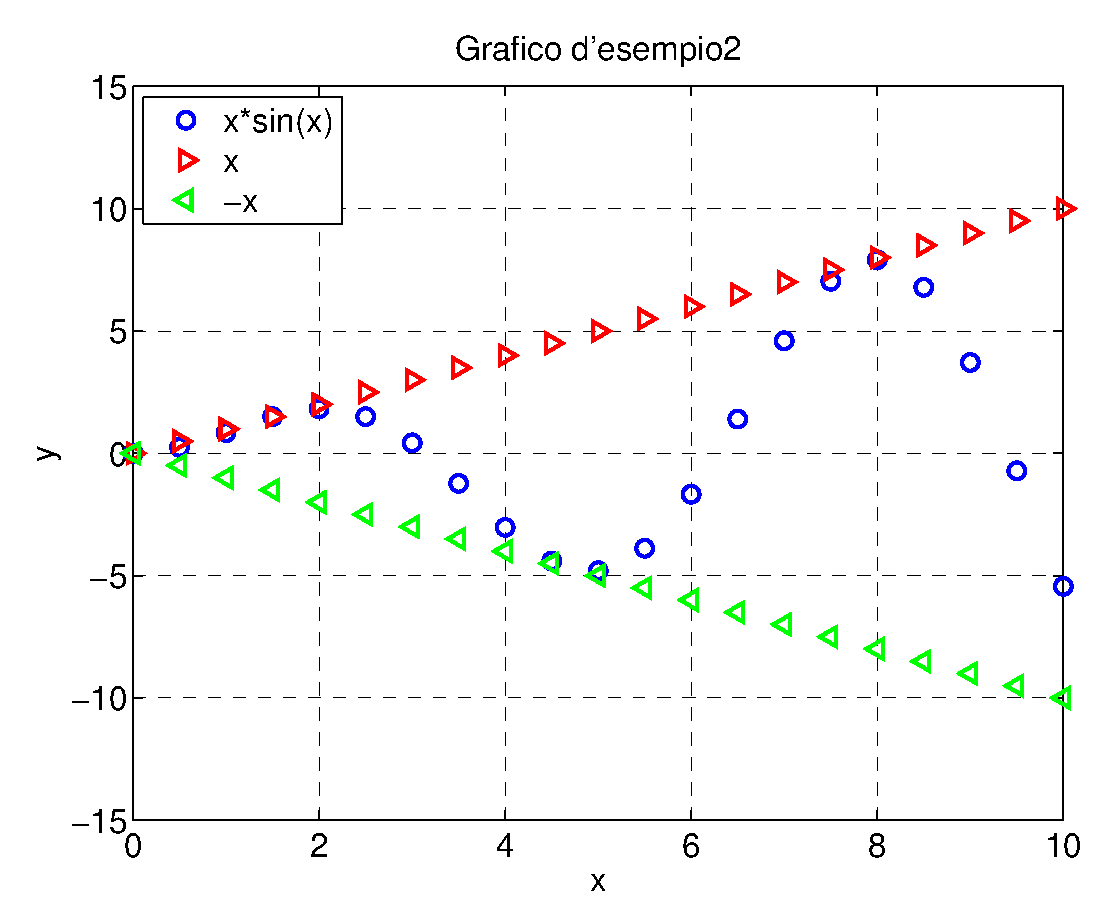
\includegraphics[width=.5\textwidth]{immagine2}}\\
%
\subfloat[][descrizione imm3\label{fig:grafici-3}]
   {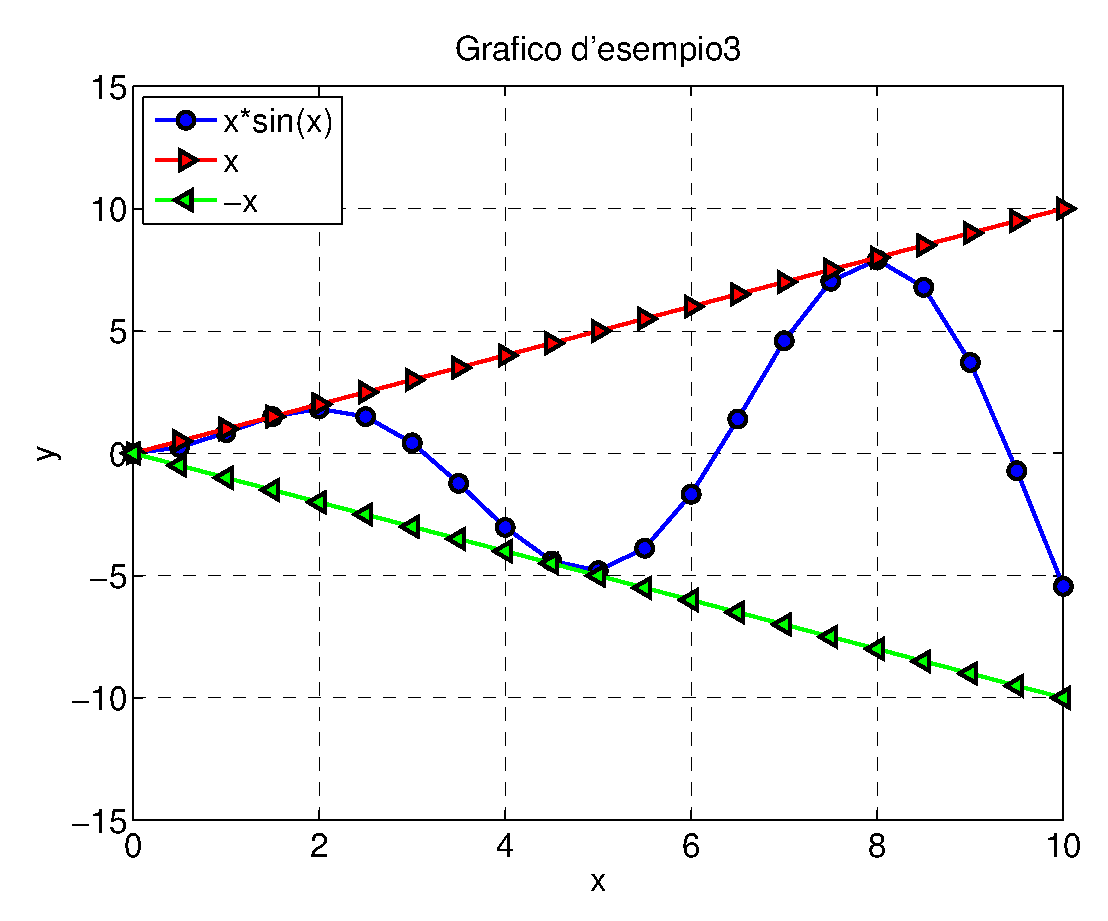
\includegraphics[width=.8\textwidth]{immagine3}}
%
\caption[Esempio di grafici]{Esempio di grafici in formato vettoriale, con griglia, box esterno e font size adeguato.}
%
\label{fig:grafici}
%
\end{figure}
%
% ------------------------------------------------------------------------ %
%
In tabella~\vref{tab:daticameraWT} sono invece riportate le principali caratteristiche (inventate) della camera di prova di una galleria del vento.
%
% TABLE
% ------------------------------------------------------------------------ %
% caratteristiche galleria del vento (inventate)
% ------------------------------------------------------------------------ %
%
\begin{table}
%
\caption{Principali caratteristiche della camera di prova utilizzata.}
%
\label{tab:daticameraWT}
%
\centering
%
\begin{tabular}{lcc}
%
\toprule
%
\multicolumn{3}{c}{\bfseries Camera Veloce a Bassa Turbolenza}\\
%
\midrule
%
Sezione Trasversale ($l$x$h$)	& [m]	& $3$x$2$ \\
Potenza Massima 		& [MW]	& \num{0.5} \\
Velocità Massima		& [m/s]	& \num{35} \\
Intensità di Turbolenza $I$ 	& [\%]	& \num{0.5} \\
%
\bottomrule
%
\end{tabular}
%
\end{table}
%
% ------------------------------------------------------------------------ %
%
\subsection{Subsection}
%
\lipsum[1-5]
%
% -----------------------------END------------------------------------- %